\chapter{System Overview} \label{overview}

Figure~\ref{fig:overview} shows the main components of Debug Support.
Blocks shown in dotted lines are optional. 

\begin{figure}
   \centering
   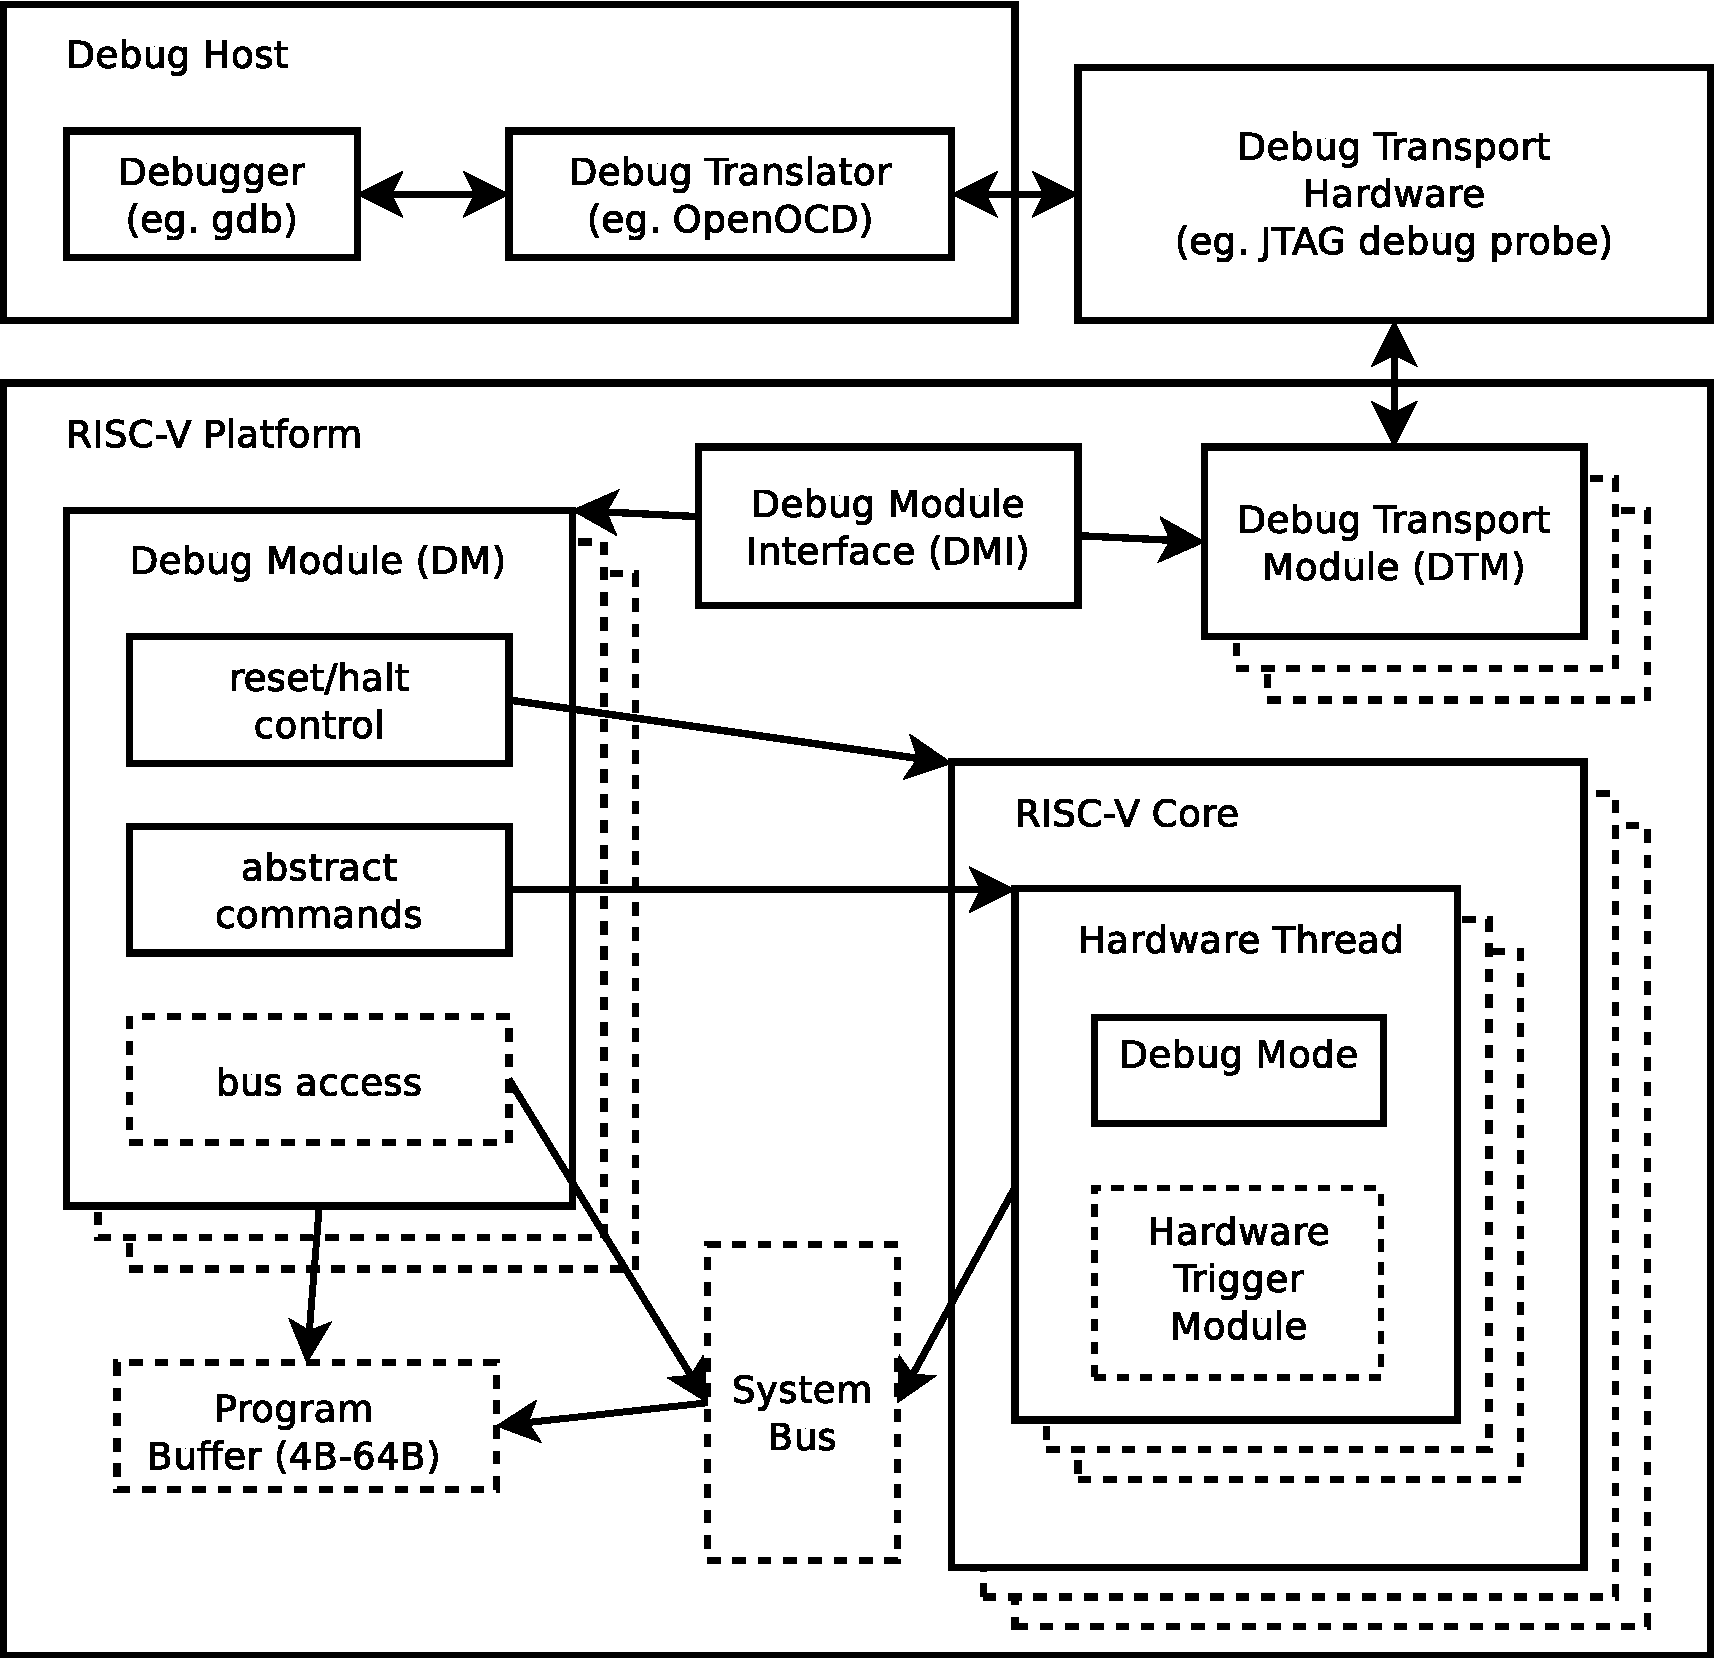
\includegraphics[width=\textwidth]{fig/overview-eps-converted-to.pdf}
   \caption{RISC-V Debug System Overview}
   \label{fig:overview}
\end{figure}

The user interacts with the Debug Host (e.g.\ laptop), which is running a
debugger (e.g.\ gdb).  The debugger communicates with a Debug Translator (e.g.\ 
OpenOCD, which may include a hardware driver) to communicate with Debug
Transport Hardware (e.g.\ Olimex USB-JTAG adapter).
The Debug Transport Hardware connects the Debug Host to the hardware platform's Debug
Transport Module (DTM).  The DTM provides access to one or more Debug Modules
(DMs) using the Debug Module Interface (DMI).

Each hart in the hardware platform is controlled by exactly one DM. Harts may be
heterogeneous. There is no further limit on the hart-DM mapping, but usually
all harts in a single core are controlled by the same DM. In most hardware platforms there
will only be one DM that controls all the harts in the hardware platform.

DMs provide run control of their harts in the hardware platform. Abstract commands
provide access to GPRs. Additional registers are accessible through abstract
commands or by writing programs to the optional Program Buffer.

The Program Buffer allows the debugger to execute arbitrary instructions on a
hart. This mechanism can also be used to access memory.  An optional system bus
access block allows memory accesses without using a RISC-V hart to perform the
access.

Each RISC-V hart may implement a Trigger Module. When trigger conditions
are met, harts will halt and inform the debug module that they have
halted.
